\section{Related Work}\label{sec:relatedWork}

Strong Branching is an efficient branching strategy in terms of the number of nodes generated but is costly in terms of time.
To mitigate the time cost disadvantage of the Strong Branching strategy, researchers have focused on developing strategies that can make Strong Branching-like decisions more quickly and efficiently.
One group of researchers aimed to leverage machine learning techniques to learn a function that would mimic the Strong Branching strategy.


\subsection{ExtraTrees Based Imitation of Strong Branching}\label{subsec:extratrees-based-imitation-of-strong-branching}
One of the pioneering studies in this field belongs to Alvarez et al.~\cite{alvarezMachineLearningBasedApproximation2017}.
In this study, Alvarez et al.~\cite{alvarezMachineLearningBasedApproximation2017} attempted to mimic the Strong Branching strategy by using a machine learning algorithm called ExtraTrees~\cite{geurtsExtremelyRandomizedTrees2006}.
The method used in this study consists of three steps.


In first step, randomly generated set covering (SC), multi knapsack (MKN), bin packing (BP), and equality (EQ) problems were solved using the Strong Branching strategy.
In addition to the Strong Branching scores calculated for each variable at each node, static problem features such as cost coefficient of variable $i$, dynamic problem features such as the fractionality of variable $i$ at the current solution and dynamic optimization features such as the number of times variable $i$ has been chosen as branching variable were also recorded for use during the training phase.
Detailed description of features can be seen in Appendix A Table 0.1. % burası revize edilecek


In second step, a function to mimic Strong Branching was learned using the ExtraTrees machine learning algorithm with $10^5$ training examples.
Alvarez et al.~\cite{alvarezMachineLearningBasedApproximation2017} approached the problem as a regression problem.
The recorded features were utilized as inputs to learn a weight vector for calculating the Strong Branching score for each branching candidate variable, in a manner similar to the Strong Branching strategy.
It can be stated that the learning process occurs offline.


In third step, the learned heuristic and other branching strategies (Random Branching, Most Infeasible Branching (MIB), Nonchimerical Branching (NCB), Full Strong Branching (FSB), and Reliability Branching (RB) were tested on two different datasets: randomly generated problems and standard benchmark problems from MIPLIB.
At this stage, two types of experiments were performed.
The first involved terminating the optimization process early, based on a predefined limit on either the number of nodes(a limit of $10^5$ nodes) explored or the computation time (a limit of 10 minutes) elapsed.
The second set of experiments allowed the problems to be solved to optimality, regardless of the time or node required.


An analysis of the experimental results, where MIPLIB problems were solved using CPLEX under node and time limits, reveals that the proposed branching strategy performs comparably to strong branching in both scenarios.
However, the performance of the learned branching strategy remains slightly inferior to that achieved with Reliability Branching (RB).
The closed gap (“Cl. Gap”) in Table~\ref{tab:alvarez-results} is defined as the ratio of the difference between the current dual bound and the objective value of the initial LP relaxation to the difference between the optimal objective value and the objective value of the initial LP relaxation.
A value close to 1 indicates that the optimization process is nearing its final stages.

\begin{table}[htb!]
    \centering
    \begin{tabular}{|c c c c c|}
        \hline
        \textbf{Criteria} & \textbf{S/T} & \textbf{Cl. Gap} & \textbf{Nodes} & \textbf{Time (s)}\\
        \hline
        \textbf{Node Limit} & & & & \\
        \textbf{Random} & 0/44 & 0.43 & 10,000 & 124.50 \\
        \textbf{MIB} & 6/44 & 0.50 & 9,274 & 233.19 \\
        \textbf{NCB} & 11/44 & 0.72 & 7,322 & 232.74\\
        \textbf{FSB} & \textbf{12/44} & \textbf{0.73} & \textbf{7,184} & 629.87 \\
        \textbf{RB} & 10/44 & 0.64 & 7,806 & 219.39 \\
        \textbf{Learned} & 10/44 & 0.62 & 8,073 & \textbf{162.87}\\
        \hline
        \textbf{Time Limit} & & & & \\
        \textbf{Random} & 0/44 & 0.47 & 867,837 & 600.01 \\
        \textbf{MIB} & 3/44 & 0.52 & 764,439 & 561.27\\
        \textbf{NCB} & 5/44 & \textbf{0.73} & 101,408 & 513.00 \\
        \textbf{FSB} & 3/44 & 0.66 & \textbf{49,008} & 534.65 \\
        \textbf{RB} & \textbf{7/44} & 0.69 & 257,375 & 515.40\\
        \textbf{Learned} & 5/44 & 0.63 & 130,081 & \textbf{512.72} \\
        \hline
    \end{tabular}
    \caption{Optimization results under node and time limits on MIBLIP dataset for different branching strategies.
    The best value is in bold.
    “S/T” represents the ratio of problems solved within the given node or time limit to the total number of problems.}
    \label{tab:alvarez-results}
\end{table}


When we examine the experimental results in which MIPLIB problems were solved by CPLEX until optimality, as can be seen in Table~\ref{tab:alvarez-results-2}, it is observed that the learned function is the strategy that produces the fastest solutions when cuts and heuristics are used by CPLEX.
It was observed that the learned function solved the problems with fewer nodes compared to the Random and MIB strategies.
However, in terms of node count, the learned function is less effective than the RB and NCB strategies.
When cuts and heuristics are not used by CPLEX learned function seems to be non-efficient in terms of node count and time.

\begin{table}[htb!]
    \centering
    \begin{tabular}{|c c c c c|}
        \hline
        \textbf{} & \multicolumn{2}{c}{\textbf{w/o cuts \& heuristics}} & \multicolumn{2}{c|}{\textbf{cuts \& heuristics}}\\
        \hline
        \textbf{Strategy} & \textbf{Nodes} & \textbf{Time(s)} & \textbf{Nodes} & \textbf{Time(s)} \\
        \hline
        \textbf{Random} & 7,809,341 & 29,377.10 & 152,564 & 503.38 \\
        \textbf{MIB} & 3,472,431 & 7,387.09 & 105,692 & 356.52 \\
        \textbf{NCB} & 145,244 & 1,136.34 & 34,500 & 1,451.74\\
        \textbf{FSB} & \textbf{129,047} & 1,597.12 & \textbf{25,941} & 895.36\\
        \textbf{RB} & 318,384 & \textbf{886.12} & 51,913 & 2,836.93\\
        \textbf{Learned} & 1,037,055 & 3,023.4 & 57,652 & \textbf{124.94}\\
        \hline
    \end{tabular}
    \caption{Optimization results (until termination) on MIBLIP dataset for different branching strategies.
    Lower is better, and the best value is in bold.}
    \label{tab:alvarez-results-2}
\end{table}


\subsection{ExtraTrees Based Imitation of Strong Branching}
Another study in this field was conducted by Khalil et al~\cite{khalilLearningBranchMixed2016}.
In this study, the researchers attempted to mimic the Strong Branching strategy using the svmRank machine learning algorithm.
This study consists of three steps.


In first step, unlike the study by Alvarez et al.~\cite{alvarezMachineLearningBasedApproximation2017}, in this research, training and testing were conducted on the same problem instance.
It can be stated that the learning process occurs online.
Branching was performed using Strong Branching for the first $\Theta$ nodes of each problem.
Each variable was assigned a label based on the Strong Branching score.
The following formula was used for label assignment:

\[ y_i^n = \begin{cases}
      1 & S_i^n\geq (1-\alpha)S_*^n \\
      0 & otherwise
   \end{cases}
\]

where $S_*^n$ is maximum SB score and the parameter $\alpha$ $\in$ [0, 1] represents the fraction of the maximum Strong Branching ($S_*^n$) that a variable must achieve to be assigned a label of '1'.
At each node, the assigned labels and the static features such as objective function coefficients and dynamic features such as the fractionality of variable i at the current solution were recorded as training data.
Detailed description of features can be seen in Appendix A Table 0.2. % burası revize edilecek


In second step, unlike Alvarez et al.~\cite{alvarezMachineLearningBasedApproximation2017}, Khalil et al.~\cite{khalilLearningBranchMixed2016} approached the problem as a ranking problem.
Instead of predicting the Strong Branching score as Alvarez et al.~\cite{alvarezMachineLearningBasedApproximation2017} did, the researchers focused on ranking the variables among themselves in a manner similar to Strong Branching.
According to the researchers, the exact Strong Branching score is not important; what matters is that the variables are ranked among themselves in the way Strong Branching would.
At this stage, a linear function ($f$) was learned using the svmRank~\cite{joachimsTrainingLinearSVMs2006} machine learning algorithm and Pairwise loss~\cite{joachimsOptimizingSearchEngines}:

\[
f: \mathbb{R}^p \rightarrow \mathbb{R}, \quad
f\left(\Phi(x_i, N_n)\right) = \mathbf{w}^T \Phi(x_i, N_n), \quad
\]

\[
\hat{y}_i^n = f\left(\Phi(x_i, N_n)\right),
\]

\[
\mathbf{w}^* = \arg\min_{\mathbf{w} \in \mathbb{R}^p}
\sum_{N_n \in N} \ell(\mathbf{y}^n, \hat{\mathbf{y}}^n)
+ \lambda \| \mathbf{w} \|_2^2
\]

where $\Phi(x_i, N_n)$ denotes variable $x_i$ at node $N_n$ with $p$ features, $\mathbf{w}^*$ denotes learned weight vector, $\ell$ denotes the loss function (Pairwise loss), $\lambda$ denotes regularization parameter that helps to avoid overfitting, $\hat{\mathbf{y}}^n$ denotes vector of values resulting from applying $f$ to every fractional variable in $N_n$, $\mathbf{y}^n$ denotes the true label of every fractional variable in $N_n$.


In third step, the learned weight vector was used for branching instead of Strong Branching.
The feature vectors of the variables were multiplied by the learned weight vector to calculate a score for each variable.
The variable with the highest score was selected for branching.


In the experimental phase, the developed method (SB+ML) was tested on MIPLIB2010 problems.
The results were compared with CPLEX's default branching strategy (CPLEX-D), Strong Branching (SB), Pseudocost Branching (PC), and the SB + PC strategy. SB+PC is a hybrid approach that uses SB for the first $\Theta$ = 500 nodes, and PC afterward.
Experiments were conducted on a total of 523 problems.
Problems solved by CPLEX-D with fewer than 50,000 nodes were classified as Easy, those solved with more than 50,000 but fewer than 500,000 nodes as Medium, and those solved with more than 500,000 nodes as Hard.
The experimental results are summarized in the Table~\ref{tab:khalil-results}:

\begin{table}[ht]
\centering
\small
\begin{tabular}{|lcccccc|}
\toprule
 & \textbf{CPLEX-D} & \textbf{SB} & \textbf{PC} & \textbf{SB+PC} & \textbf{SB+ML} \\
\midrule
\textbf{Unsolved} & & & & & \\
\textbf{Instances} & & & & & \\
\quad All (523) & 11 & 129 & 66 & 63 & \textbf{52} \\
\quad Easy (255) & 0 & 12 & 15 & 14 & \textbf{13} \\
\quad Medium (120) & 2 & 43 & 22 & 22 & \textbf{17} \\
\quad Hard (148) & 9 & 74 & 29 & 27 & \textbf{22} \\
\midrule
\textbf{Number of} & & & & & \\
\textbf{Nodes} & & & & & \\
\quad All (523) & 46,633 & 33,072 & 92,662 & 70,455 & \textbf{59,223} \\
\quad Easy (255) & 3,255 & 3,610 & 7,931 & 5,224 & \textbf{5,124} \\
\quad Medium (120) & 173,417 & 121,923 & 395,199 & 288,916 & \textbf{234,093} \\
\quad Hard (148) & 1,570,891 & 519,878 & 1,971,333 & 1,979,660 & \textbf{1,314,263} \\
\midrule
\textbf{Total Time} & & & & & \\
\textbf{(s)} & & & & & \\
\quad All (523) & 499 & 2,263 & \textbf{960} & 1,093 & 1,059 \\
\quad Easy (255) & 111 & 602 & \textbf{243} & 361 & 382 \\
\quad Medium (120) & 1,123 & 6,169 & 2,493 & 1,892 & \textbf{1,776} \\
\quad Hard (148) & 3,421 & 9,803 & 4,705 & 4,718 & \textbf{4,039} \\
\bottomrule
\end{tabular}
\caption{“Unsolved instances” are counts, “Num. nodes” and “Total time” (in seconds) are shifted geometric means over instances with shifts 10 and 1, respectively.
Lower is better, and the best value in each row among PC, SB+PC and SB+ML is in bold.}
    \label{tab:khalil-results}
\end{table}


The researchers analyzed the experimental results from three perspectives: the number of unsolved problems, the total number of nodes, and the total solution time.
Since the researchers claimed that the developed method is better at selecting branching variables, the primary metric they focused on was the total number of nodes.
As can be seen from the table above, the developed method (SB+ML) is more successful in terms of the total number of nodes compared to PC and SB+PC.
When considering all the problems, it was observed that the developed method reduced the solution time compared to the Strong Branching strategy, while increasing the number of nodes.


\subsection{GCNN Based Imitation of Strong Branching}\label{subsec:gcnn-based-imitation-of-strong-branching}
In another study in this field, Gasse et al.~\cite{gasseExactCombinatorialOptimization2019} attempted to mimic the Strong Branching strategy using a Graph Convolutional Neural Network (GCNN).
In this study, the researchers used the bipartite graph representation of MILP problems, enabling the use of GCNN in solving MILP problems.
This study consists of three steps.


In first step, 100,000 branching examples were collected from 10,000 randomly generated MILP problems (Set Covering Problems, Combinatorial Auction Problems,Capacitated Facility Location Problems, Maximum Independent Set Problems).
For each branching example, the Strong Branching scores calculated for the variables and variable features such as objective coefficient, constraint features such as dual solution value, edge features such as constraint coefficient were collected.
Detailed description of features can be seen in Appendix A Table 0.3. % burası revize edilecek


In second step, unlike Alvarez et al.~\cite{alvarezMachineLearningBasedApproximation2017} and Khalil et al.~\cite{khalilLearningBranchMixed2016}, Gasse et al.~\cite{gasseExactCombinatorialOptimization2019} approached the problem as a classification problem.
They attempted to learn how to select the variable to be used in branching with a Graph Neural Network, mimicking the approach of the Strong Branching strategy.
The GNN architecture used here essentially consists of three components as can be seen in Figure~\ref{fig:gcnn}.

\begin{figure*}[htb!]
    \centering
    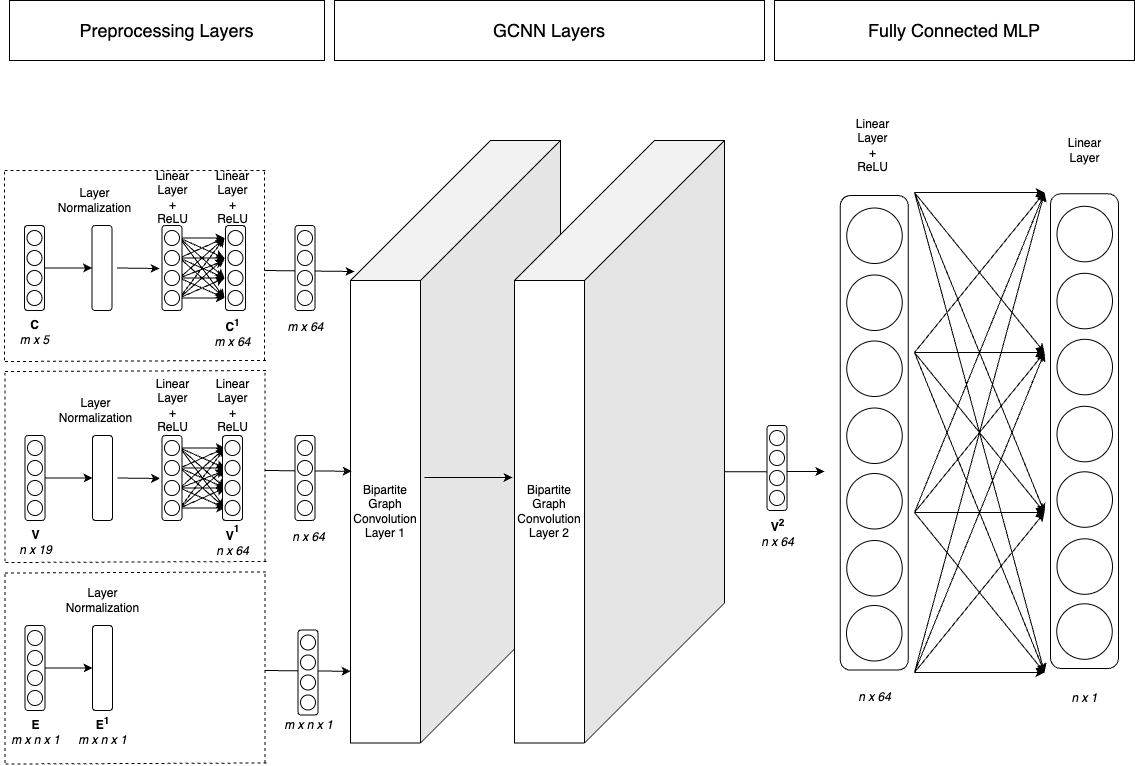
\includegraphics[width=1\textwidth]{figures/GCNN}
    \caption{GNN architecture developed by Gasse et al.~\cite{gasseExactCombinatorialOptimization2019}.}
    \label{fig:gcnn}
\end{figure*}


\begin{itemize}
  \item Preprocessing Layers: At this stage, the constraint features and variable features are transformed into 64-dimensional embeddings using a fully connected 2-layer MLP with layer normalization~\cite{baLayerNormalization2016} and ReLU activation function.
  Layer normalization is applied to the edge features.
  \item GCNN Layers: The variable, constraint, and edge features undergo convolution operations twice.
  The researchers developed a custom convolution operator called Bipartite Graph Convolution for this process, the details of which are shown in Figure~\ref{fig:convolution}.
  \item Fully Connected MLP: At this stage, the variable embeddings, which have undergone two convolution operations, are passed through a 2-layer MLP.
  A ReLU activation function is used in the first layer, A SoftMax activation function is used in the second layer.
  As a result of this process, the 64-dimensional embeddings for each variable are converted into a single-dimensional score.
\end{itemize}


The developed GNN architecture was trained on 100,000 branching examples using the Adam Optimizer~\cite{kingmaAdamMethodStochastic2017} and Cross Entropy Loss.

\begin{figure*}[htb!]
    \centering
    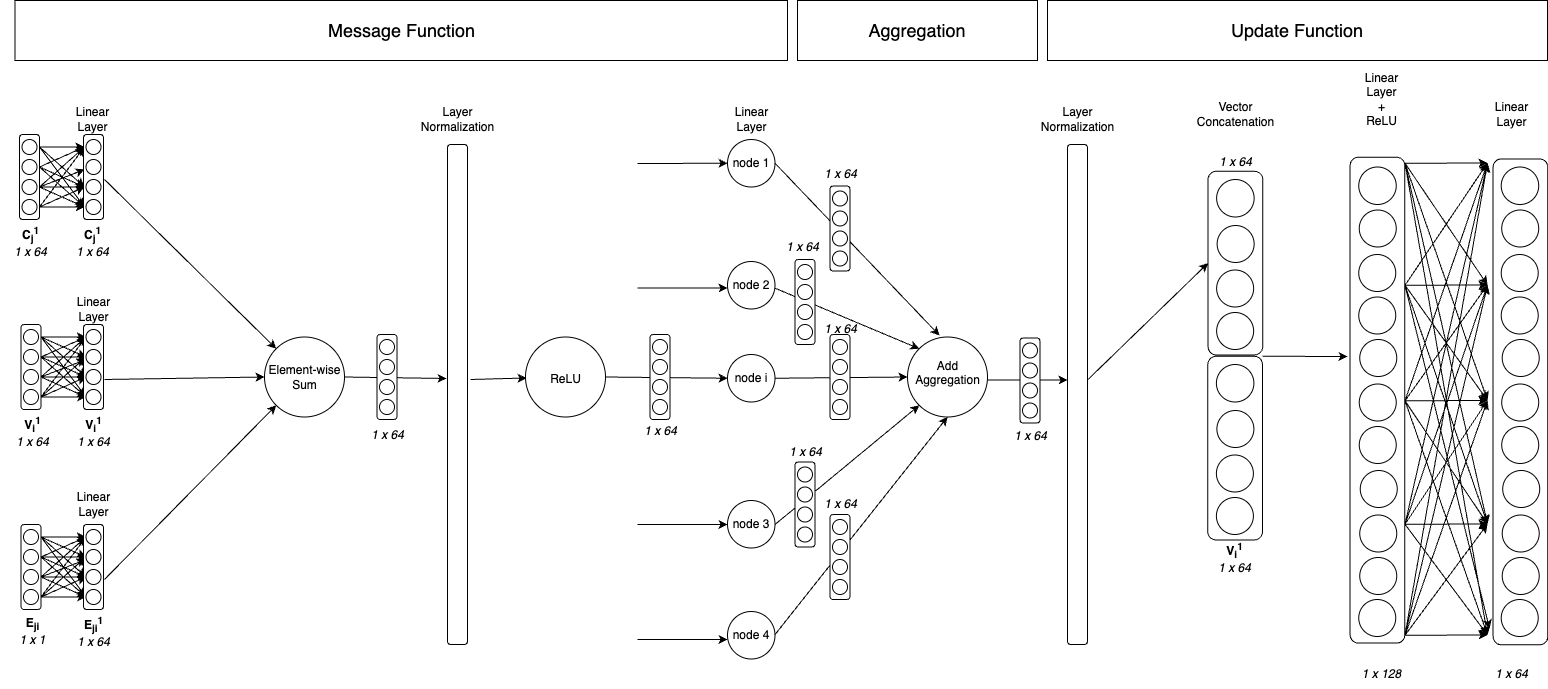
\includegraphics[width=1\textwidth]{figures/Convolution}
    \caption{Bipartite Graph Convolution Layer developed by Gasse et al.~\cite{gasseExactCombinatorialOptimization2019}.}
    \label{fig:convolution}
\end{figure*}


In third step, Gasse et al.~\cite{gasseExactCombinatorialOptimization2019}'s developed model was compared with Full Strong Branching (FSB), Reliability Pseudocost Branching (RPB), the ExtraTrees method developed by Alvarez et al.~\cite{alvarezMachineLearningBasedApproximation2017} (TREES), LambdaMART method developed by Hansknecht et al.~\cite{hansknechtCutsPrimalHeuristics2018a} (LMART) and the svmRank method developed by Khalil et al.~\cite{khalilLearningBranchMixed2016} (SVMRANK) using 100 easy, 100 medium, 100 hard problems.
Problem parameters can be seen in Table~\ref{tab:gasse-benchmark-problems}.

\begin{table*}[htb!]
    \centering
    \begin{tabular}{|l c c c|}
        \hline
        \textbf{Problem Type} & \textbf{Easy} & \textbf{Medium} & \textbf{Hard}\\
        \hline
        \textbf{Set Covering~\cite{balasSetCoveringAlgorithms1980}} & 500 rows, 1000 columns & 1000 rows, 1000 columns & 2000 rows, 1000 columns\\
        \textbf{Combinatorial Auction~\cite{leyton-brownUniversalTestSuite2000}} & 100 items for 500 bids & 200 items for 1000 bids & 300 items for 1500 bids\\
        \textbf{Capacitated Facility Location~\cite{cornuejolsComparisonHeuristicsRelaxations1991}} & 100 customers & 200 customers & 400 customers\\
        \textbf{Maximum Independent Set~\cite{bergmanDecisionDiagramsOptimization2016}} & 500 nodes & 1000 nodes & 1500 nodes\\
        \hline
    \end{tabular}
    \caption{Four NP-hard problem benchmarks used for evaluation by Gasse et al.~\cite{gasseExactCombinatorialOptimization2019}.}
    \label{tab:gasse-benchmark-problems}
\end{table*}


The performance of different branching methods was evaluated based on the number of nodes required to solve instances and the overall solving time, which includes the computational cost of branching policies such as feature extraction and inference.
As can be seen from the Table~\ref{tab:gasse-results}, The GCNN model demonstrated superior performance overall, particularly excelling in generalizing to larger instances and outperforming SCIP's default RPB branching rule in nearly all configurations, especially on medium and hard instances of set cover and combinatorial auction problems.
However, it faced challenges with the maximum independent set problem, showing high variability in both runtime and node count.


Although the FSB expert brancher produced small search trees, it was not competitive in runtime.
The study marks the first comparison of a machine learning-based method with a comprehensive MILP solver, highlighting GCNN's potential as a promising addition to MILP solvers for accelerating mixed-integer linear programming tasks.
These findings suggest that tighter integration of GCNN within a MILP solver could unlock further improvements.

\begin{table*}[htb!]
    \centering
    \begin{footnotesize}
    \begin{tabular}{|l c c c c c c c c c|}
        \hline
        \textbf{} & \multicolumn{3}{c}{\textbf{Easy}} & \multicolumn{3}{c}{\textbf{Medium}} & \multicolumn{3}{c|}{\textbf{Hard}}\\
        \hline
        \textbf{Model} & \textbf{Time} & \textbf{Wins} & \textbf{Nodes} & \textbf{Time} & \textbf{Wins} & \textbf{Nodes} & \textbf{Time} & \textbf{Wins} & \textbf{Nodes} \\
        \hline
        \textbf{FSB} & 17.30$\pm$6.1\% & 0/100 & 17$\pm$13.7\% & 411.34$\pm$4.3\% & 0/90 & 171$\pm$6.4\% & 3600.00$\pm$0.0\% & 0/0 & n/a$\pm$n/a\%\\
        \textbf{RPB} & 8.98$\pm$4.8\% & 0/100 & \textbf{54}$\pm$20.8\% & 60.07$\pm$3.7\% & 0/100 & 1741$\pm$7.9\% & 1677.02$\pm$3.0\% & 4/65 & 47299$\pm$4.9\%\\
        \textbf{TREES} & 9.28$\pm$4.9\% & 0/100 & 187$\pm$9.4\% & 92.47$\pm$5.9\% & 0/100 & 2187$\pm$7.9\% & 2869.21$\pm$3.2\% & 0/35 & 59013$\pm$9.3\%\\
        \textbf{SVMRANK} & 8.10$\pm$3.8\% & 1/100 & 165$\pm$8.2\% & 73.58$\pm$3.1\% & 0/100 & 1915$\pm$3.8\% & 2389.92$\pm$2.3\% & 0/47 & 42120$\pm$5.4\%\\
        \textbf{LMART} & 7.19$\pm$4.2\% & 14/100 & 167$\pm$9.0\% & 59.98$\pm$3.9\% & 0/100 & 1925$\pm$4.9\% & 2165.96$\pm$2.0\% & 0/54 & 45319$\pm$3.4\%\\
        \textbf{GCNN} & \textbf{6.59}$\pm$3.1\% & \textbf{85}/100 & 134$\pm$7.6\% & \textbf{42.48}$\pm$2.7\% & \textbf{100}/100 & \textbf{1450}$\pm$3.3\% & \textbf{1489.91}$\pm$3.3\% & \textbf{66}/70 & \textbf{29981}$\pm$4.9\%\\
        \multicolumn{10}{|c|}{\textbf{Set Covering}}\\
        \hline
        \textbf{FSB} & 4.11$\pm$12.1\% & 0/100 & 6$\pm$30.3\% & 86.90$\pm$12.9\% & 0/100 & 72$\pm$19.4\% & 1813.33$\pm$5.1\% & 0/68 & 400$\pm$7.5\%\\
        \textbf{RPB} & 2.74$\pm$7.8\% & 0/100 & \textbf{10}$\pm$32.1\% & 17.41$\pm$6.6\% & 0/100 & 689$\pm$21.2\% & 136.17$\pm$7.9\% & 13/100 & 5511$\pm$11.7\%\\
        \textbf{TREES} & 2.47$\pm$7.3\% & 0/100 & 86$\pm$15.9\% & 23.30$\pm$11.2\% & 0/100 & 976$\pm$14.4\% & 451.39$\pm$14.6\% & 0/95 & 10290$\pm$16.2\%\\
        \textbf{SVMRANK} & 2.31$\pm$6.8\% & 0/100 & 77$\pm$15.0\% & 23.10$\pm$9.8\% & 0/100 & 867$\pm$13.4\% & 364.48$\pm$7.7\% & 0/98 & 6329$\pm$7.7\%\\
        \textbf{LMART} & \textbf{1.79}$\pm$6.0\% & \textbf{75}/100 & 77$\pm$14.9\% & 14.42$\pm$9.5\% & 1/100 & 873$\pm$14.3\% & 222.54$\pm$8.6\% & 0/100 & 7006$\pm$6.9\%\\
        \textbf{GCNN} & 1.85$\pm$5.0\% & 25/100 & 70$\pm$12.0\% & \textbf{10.29}$\pm$7.1\% & \textbf{99}/100 & \textbf{657}$\pm$12.2\% & \textbf{114.16}$\pm$10.3\% & \textbf{87}/100 & \textbf{5169}$\pm$14.9\%\\
        \multicolumn{10}{|c|}{\textbf{Combinatorial Auction}}\\
        \hline
        \textbf{FSB} & 30.36$\pm$19.6\% & 4/100 & 14$\pm$34.5\% & 214.25$\pm$15.2\% & 1/100 & 76$\pm$15.8\% & 742.91$\pm$9.1\% & 15/90 & 55$\pm$7.2\%\\
        \textbf{RPB} & 26.55$\pm$16.2\% & 9/100 & \textbf{22}$\pm$31.9\% & 156.12$\pm$11.5\% & 8/100 & \textbf{142}$\pm$20.6\% & 631.50$\pm$8.1\% & 14/96 & \textbf{110}$\pm$15.5\%\\
        \textbf{TREES} & 28.96$\pm$14.7\% & 3/100 & 135$\pm$20.0\% & 159.86$\pm$15.3\% & 3/100 & 401$\pm$11.6\% & 671.01$\pm$11.1\% & 1/95 & 381$\pm$11.1\%\\
        \textbf{SVMRANK} & 23.58$\pm$14.1\% & 11/100 & 117$\pm$20.5\% & 130.86$\pm$13.6\% & 13/100 & 348$\pm$11.4\% & 586.13$\pm$10.0\% & 21/95 & 321$\pm$8.8\%\\
        \textbf{LMART} & 23.34$\pm$13.6\% & 16/100 & 117$\pm$20.7\% & 128.48$\pm$15.4\% & 23/100 & 349$\pm$12.9\% & 582.38$\pm$10.5\% & 15/95 & 314$\pm$7.0\%\\
        \textbf{GCNN} & \textbf{22.10}$\pm$15.8\% & \textbf{57}/100 & 107$\pm$21.4\% & \textbf{120.94}$\pm$14.2\% & \textbf{52}/100 & 339$\pm$11.8\% & \textbf{563.36}$\pm$10.7\% & \textbf{30}/95 & 338$\pm$10.9\%\\
        \multicolumn{10}{|c|}{\textbf{Capacitated Facility Location}}\\
        \hline
        \textbf{FSB} & 23.58$\pm$29.9\% & 9/100 & 7$\pm$35.9\% & 1503.55$\pm$20.9\% & 0/74 & 38$\pm$28.2\% & 3600.00$\pm$0.0\% & 0/0 & n/a$\pm$n/a\%\\
        \textbf{RPB} & 8.77$\pm$11.8\% & 7/100 & \textbf{20}$\pm$36.1\% & \textbf{110.99}$\pm$24.4\% & 41/100 & \textbf{729}$\pm$37.3\% & 2045.61$\pm$18.3\% & 22/42 & \textbf{2675}$\pm$24.10\%\\
        \textbf{TREES} & 10.75$\pm$22.1\% & 1/100 & 76$\pm$44.2\% & 1183.37$\pm$34.2\% & 1/47 & 4664$\pm$45.8\% & 3565.12$\pm$1.2\% & 0/3 & 38296$\pm$4.1\%\\
        \textbf{SVMRANK} & 8.83$\pm$14.9\% & 2/100 & 46$\pm$32.2\% & 242.91$\pm$29.3\% & 1/96 & 546$\pm$26.0\% & 2902.94$\pm$9.6\% & 1/18 & 6256$\pm$15.1\%\\
        \textbf{LMART} & 7.31$\pm$12.7\% & 30/100 & 52$\pm$38.1\% & 219.22$\pm$36.0\% & 15/91 & 747$\pm$35.1\% & 3044.94$\pm$7.0\% & 0/12 & 8893$\pm$3.5\%\\
        \textbf{GCNN} & \textbf{6.43}$\pm$11.6\% & \textbf{51}/100 & 43$\pm$40.2\% & 192.91$\pm$110.2\% & \textbf{42}/82 & 1841$\pm$88.0\% & \textbf{2024.37}$\pm$30.6\% & \textbf{25}/29 & 2997$\pm$26.3\%\\
        \multicolumn{10}{|c|}{\textbf{Maximum Independent Set}}\\
        \hline
    \end{tabular}
    \end{footnotesize}
    \caption{Policy evaluation was conducted on Set Covering, Combinatorial Auction, Capacitated Facility Location, and Maximum Independent Set instances, focusing on solving time, the number of wins (i.e., the fastest method) relative to the number of solved instances, and the number of resulting B\&B nodes (with lower values being preferable).
    For each problem, the models were trained exclusively on easy instances.}
    \label{tab:gasse-results}
\end{table*}

\subsection{The Distinction of Study from Previous Works}
In this study, unlike the approaches of Alvarez et al.~\cite{alvarezMachineLearningBasedApproximation2017} and Khalil et al.~\cite{khalilLearningBranchMixed2016}, the problem is formulated as a classification task.
According to the Universal Approximation Theorem~\cite{luUniversalApproximationTheorem2020}, it is theoretically possible to approximate any function given a sufficient number of neurons.
To leverage the high learning capacity of neural networks, this study employs Graph Neural Networks (GNNs) as the machine learning algorithm, as was done in the study by Gasse et al.~\cite{gasseExactCombinatorialOptimization2019}.
Gasse et al.~\cite{gasseExactCombinatorialOptimization2019} demonstrated in their research that the Graph Neural Network algorithm achieves superior performance compared to alternative methods such as Alvarez et al.~\cite{alvarezMachineLearningBasedApproximation2017}’s ExtraTrees algorithm and Khalil et al.~\cite{khalilLearningBranchMixed2016}’s SVMRank algorithm.


The key point of divergence between this study and the work of Gasse et al.~\cite{gasseExactCombinatorialOptimization2019} lies in the design of the convolutional layers utilized in the GNN architecture.
In the Graph Convolutional Neural Network (GCNN) architecture, all neighboring nodes are treated with equal significance when aggregating information for a given node.
However, this assumption often does not hold true for most real-world problems, where the importance of neighboring nodes varies.
To address this limitation, the Graph Attention Network (GAT) architecture introduces an attention mechanism that assigns varying levels of importance to neighboring nodes.
By learning adaptive weights for these neighbors, GAT provides a more nuanced representation of node relationships.


This ability to differentiate the significance of neighbors makes GAT a promising candidate for solving combinatorial optimization problems more effectively than GCNN.
This modification is aimed at further enhancing the model's ability to effectively address the underlying problem, highlighting the novelty of the proposed approach.